% fig-pilot-scores.tex
% Combined strip plot: per-run scores (10 runs) across the three rubric
% dimensions, Cond A (SmartKit) vs Cond B (convention-naive scaffold),
% with a short horizontal tick marking each condition's median.
% Requires \usepackage{pgfplots} and \pgfplotsset{compat=1.18} in the
% main preamble (added in the same commit that adds this figure).

\definecolor{dim1}{RGB}{0,90,181}   % Cond A - blue
\definecolor{dim2}{RGB}{216,84,26}  % Cond B - orange-red

\begin{figure}[H]
\centering
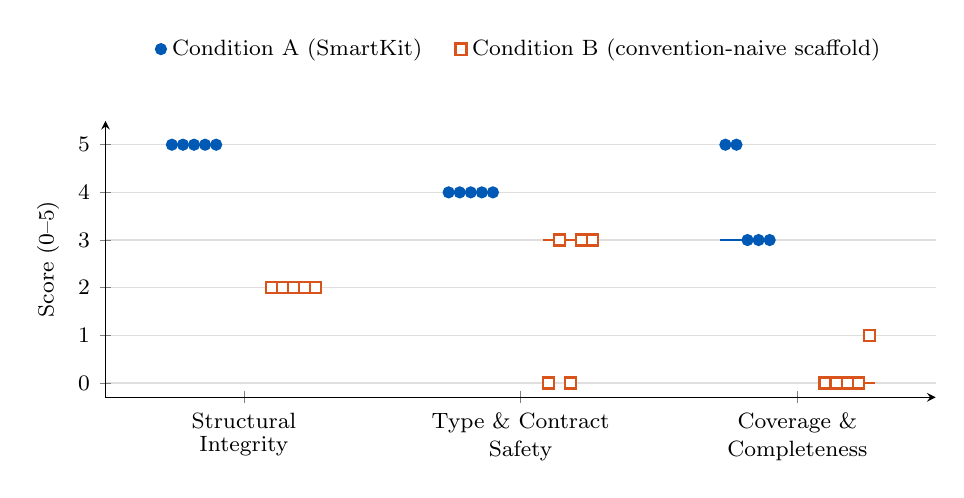
\begin{tikzpicture}
\begin{axis}[
    width=\linewidth,
    height=0.42\linewidth,
    ymin=-0.3, ymax=5.5,
    xmin=0.5, xmax=3.5,
    ytick={0,1,2,3,4,5},
    ylabel={Score (0--5)},
    xtick={1,2,3},
    xticklabels={
        {\shortstack{Structural\\Integrity}},
        {\shortstack{Type \& Contract\\Safety}},
        {\shortstack{Coverage \&\\Completeness}}
    },
    xticklabel style={align=center, font=\footnotesize},
    tick label style={font=\footnotesize},
    label style={font=\footnotesize},
    axis lines=left,
    ymajorgrids=true,
    grid style={gray!25},
    legend style={
        at={(0.5,1.18)}, anchor=south, legend columns=2,
        font=\footnotesize, draw=none,
        /tikz/every even column/.append style={column sep=10pt}
    },
    clip=false,
]

% --- Condition A (SmartKit), n=5 per dimension, filled circles ---
% Points within a cluster are jittered horizontally purely for visibility
% (runs land on integer scores; the x-position within a cluster carries no
% meaning). Structural Integrity: all 5 runs at 5. Type & Contract Safety:
% all 5 runs at 4. Coverage & Completeness: raw (pre-cap) scores are
% {5, 5, 3, 3, 3} (run-06, run-07 uncap-triggered; run-08, run-09, run-10
% cap-triggered); the cluster's median is 3 with two runs at 5 and three
% at 3. The cap is a measurement correction (per-user override stub
% detector); see \autoref{sec:integrations-and-pilot}.
\addplot[only marks, mark=*, mark size=2pt,
    mark options={fill=dim1, draw=dim1}] coordinates {
    (0.74,5) (0.78,5) (0.82,5) (0.86,5) (0.90,5)   % Structural Integrity, Runs 6-10
    (1.74,4) (1.78,4) (1.82,4) (1.86,4) (1.90,4)   % Type & Contract Safety, Runs 6-10
    (2.74,5) (2.78,5) (2.82,3) (2.86,3) (2.90,3)   % Coverage & Completeness, Runs 6-10 (raw; {5,5,3,3,3})
};
\addlegendentry{Condition~A (SmartKit)}

% --- Condition B (convention-naive scaffold), n=5 per dimension, open squares ---
% Per-run scores (in run order 1-5): Structural Integrity all 2;
% Type & Contract Safety {0, 3, 0, 3, 3} (run-01 and run-03 produced no
% flags.ts file, scoring Contract=0 under the scorer's file-presence rule;
% run-02, run-04, run-05 produced flags.ts without Zod and scored Contract=3);
% Coverage & Completeness {0, 0, 0, 0, 1} (only run-05 produced a test file,
% colocated with flag.ts at the repository root, scoring Cov=1).
\addplot[only marks, mark=square*, mark size=2pt,
    mark options={fill=white, draw=dim2, line width=0.8pt}] coordinates {
    (1.10,2) (1.14,2) (1.18,2) (1.22,2) (1.26,2)   % Structural Integrity, Runs 1-5: all 2
    (2.10,0) (2.14,3) (2.18,0) (2.22,3) (2.26,3)   % Type & Contract Safety, Runs 1-5: {0,3,0,3,3}
    (3.10,0) (3.14,0) (3.18,0) (3.22,0) (3.26,1)   % Coverage & Completeness, Runs 1-5: {0,0,0,0,1}
};
\addlegendentry{Condition~B (convention-naive scaffold)}

% --- Median ticks: short horizontal bar at each cluster's median score ---
\addplot[thick, dim1, forget plot] coordinates {(0.72,5) (0.92,5)}; % Structural Integrity, Cond A median
\addplot[thick, dim2, forget plot] coordinates {(1.08,2) (1.28,2)}; % Structural Integrity, Cond B median
\addplot[thick, dim1, forget plot] coordinates {(1.72,4) (1.92,4)}; % Type & Contract Safety, Cond A median
\addplot[thick, dim2, forget plot] coordinates {(2.08,3) (2.28,3)}; % Type & Contract Safety, Cond B median
\addplot[thick, dim1, forget plot] coordinates {(2.72,3) (2.92,3)}; % Coverage & Completeness, Cond A median (capped)
\addplot[thick, dim2, forget plot] coordinates {(3.08,0) (3.28,0)}; % Coverage & Completeness, Cond B median

\end{axis}
\end{tikzpicture}
\caption{Per-run pilot scores across 10 runs and three rubric dimensions. Cond~A (SmartKit, Runs~6--10) versus Cond~B (convention-naive scaffold, Runs~1--5).}
\label{fig:pilot-scores}
\end{figure}